\documentclass[12pt, a4paper]{report} % Defines the font size and the paper format

\usepackage[utf8]{inputenc}
\usepackage[T1]{fontenc}
\usepackage{textcomp}


\usepackage{amsmath, amssymb, amsfonts} % Standard AMS packages
\usepackage{amsthm}           % For theorem environments
\usepackage{geometry}         % Customize page geometry
\usepackage{setspace}         % To set line spacing
\usepackage{graphicx}
\usepackage[ngerman, english]{babel}


\usepackage[hidelinks]{hyperref}
\usepackage{graphicx, xcolor}

\usepackage{tikz}
\usepackage{pgfplots}
\usepackage{pdflscape}

\usepackage{color}
\usepackage{xcolor}
\usepackage{listingsutf8}

\definecolor{codeBackground}{rgb}{.95,0.95,0.95}

\newcommand{\coloredlstinline}[2]{\colorbox{codeBackground}{\lstinline[language=#1]|#2|}}

\lstset{basicstyle=\ttfamily\footnotesize,breaklines=true}
\definecolor{tangoSkyBlue}{RGB}{32, 74, 135}
\definecolor{tangoOrange}{RGB}{206, 92, 0}
\definecolor{tangoChameleon}{RGB}{78, 154, 6}
\definecolor{tangoButter}{RGB}{196, 160, 0}

\lstdefinelanguage{Rust}{
	basicstyle=\normalsize\ttfamily,
	keywords=[0]{let, pub, struct, enum, type, impl, fn, const, mut, extern, use, mod, continue, break, loop, while, crate, true, false, bool, char, str, u8, i8, u16, i16, u32, i32, u64, i64, u128, i128, usize, isize, f32, f64, match, switch, if, else, return, trait, ref, unsafe, union, for, in, dyn, where, default, as, move, static},
	keywords=[1]{|, -, !, ?, \&, *, Err, Ok, None, Some, self},
%	keywords=[2]{println!, writeln!, print!, write!},
	otherkeywords={!, ?, |, -, \&, *, \_},
	morekeywords=[1]{!, ?, |, -},
	sensitive=true,
	morecomment=[l]{//},
	morecomment=[s]{/*}{*/},
	morestring=[b]',
	morestring=[b]",
	morestring=[s][\color{tangoOrange}]{'}{a},
	alsoletter={! ? | - \& * \_},
	moredelim = [l][\color{tangoOrange}]{\#}
}

\lstdefinelanguage{help}{
	basicstyle=\ttfamily\footnotesize,
	keywords=[0]{default},
	keywords=[1]{|, -, !, ?, \&, *, Err, Ok, None, Some, self},
	%	keywords=[2]{println!, writeln!, print!, write!},
	otherkeywords={!, ?, |, -, \&, *, \_},
	morekeywords=[1]{!, ?, |, -},
	sensitive=true,
	morecomment=[l]{//},
	morecomment=[s]{/*}{*/},
	morestring=[b]',
	morestring=[b]",
	morestring=[s][\color{tangoOrange}]{'}{a},
	alsoletter={! ? | - \& * \_},
	moredelim = [l][\color{tangoOrange}]{\#}
}

%\usepackage{sourcecodepro}
%\usepackage{fontspec}
%\setmonofont{CMU Typewriter Text}
\lstset{
	backgroundcolor=\color{codeBackground},
	basicstyle=\ttfamily,
	breakatwhitespace=false,
	breaklines=true,
	captionpos=b,
	extendedchars=true,
	language=Rust,
	keywordstyle=\bf,
	showspaces=false,
    showstringspaces=false,
	showtabs=false,
	tabsize=4,
	aboveskip=5mm,
	belowskip=5mm,
	numbers=left,
	numberstyle=\tiny\color{gray},
	keywordstyle=[0]\bfseries\color{tangoSkyBlue},
	keywordstyle=[1]\bfseries\color{tangoOrange},
	keywordstyle=[2]\bfseries\color{tangoButter},
	commentstyle=\color{gray},
	stringstyle=\color{tangoChameleon},
	extendedchars=true,
	literate={ä}{{\"{a}}}1 {ö}{{\"{o}}}1 {ü}{{\"{u}}}1 {ß}{{\ss}}1,
	columns=fixed,
	keepspaces=true,
	breaklines=true,
	breakatwhitespace=true
}
\lstset{
	backgroundcolor=\color{codeBackground},
	breakatwhitespace=false,
	breaklines=true,
	captionpos=b,
	extendedchars=true,
	language=help,
	keywordstyle=\bf,
	showspaces=false,
	showstringspaces=false,
	showtabs=false,
	tabsize=4,
	aboveskip=5mm,
	belowskip=5mm,
	numbers=left,
	numberstyle=\tiny\color{gray},
	keywordstyle=[0]\bfseries\color{tangoSkyBlue},
	keywordstyle=[1]\bfseries\color{tangoOrange},
	keywordstyle=[2]\bfseries\color{tangoButter},
	commentstyle=\color{gray},
	stringstyle=\color{tangoChameleon},
	extendedchars=true,
	literate={ä}{{\"{a}}}1 {ö}{{\"{o}}}1 {ü}{{\"{u}}}1 {ß}{{\ss}}1,
	columns=fixed,
	keepspaces=true,
	breaklines=true,
	breakatwhitespace=true
}


\newcommand{\coloredlstinlinev}[2]{\colorbox{codeBackground}{\lstinline[language=#1]|#2|}}
\newcommand{\rustcinline}[1]{\coloredlstinline{rust}{#1}}
\newcommand{\rustcinclude}[3]{\lstinputlisting[language=rust,caption={#2},label={#1}]{#3}}
\newcommand{\rustcincludeml}[3]{\lstinputlisting[xleftmargin=1.2em,language=rust,caption=#2,label=#1]{#3}}

\newcommand{\helpinclude}[3]{\lstinputlisting[language=help,caption={#2},label={#1}]{#3}}

\newcommand{\javacinline}[1]{\coloredlstinline{java}{#1}}
\newcommand{\javacinclude}[3]{\lstinputlisting[language=java,caption={#2},label={#1}]{#3}}

\newcommand{\cscinline}[1]{\coloredlstinline{{[Sharp]C}}{#1}}

\newcommand{\ccinline}[1]{\coloredlstinline{c}{#1}}
\newcommand{\ccinclude}[3]{\lstinputlisting[language=c,caption={#2},label={#1}]{#3}}
\newcommand{\ccincludeml}[3]{\lstinputlisting[xleftmargin=1.2em,language=c,caption=#2,label=#1]{#3}}

\newcommand{\monospaceinclude}[3]{\lstinputlisting[basicstyle=\footnotesize,language=bash,caption=#2,label=#1]{#3}}
\newcommand{\monospaceinline}[1]{\coloredlstinline{bash}{#1}}
%\renewenvironment{rustc}{\begin{lstlisting}[language=rust]}{\end{lstlisting}}



%--------------------------------------------------------------------
%--- Title, author, date
%--------------------------------------------------------------------

\newcommand{\theuniversity}{
  \begin{figure}[h]
    \centering
    
\includegraphics[width=.5\textwidth]{brunel.jpg}
  \end{figure}}
\newcommand{\thecollege}{College of Engineering, Design and Physical Sciences, Electronic and Computer Engineering}
\newcommand{\thedepartment}{Distributed Computing Systems Engineering}
%\newcommand{\thecoursetitle}{Master Thesis - Interim Report}
\newcommand{\thecoursetitle}{Interim Report}
\newcommand{\thestudent}{Michael Watzko}
\newcommand{\thestudentid}{1841795}
\newcommand{\thesupervisor}{Dr. Paul Kyberd}
\newcommand{\theyear}{2019}
\newcommand{\thetitle}{ Conception and realization of a distributed and automated computer vision pipeline}
\newcommand{\todo}[1]{\textcolor{red}{TODO: #1}}

%--------------------------------------------------------------------
%--- Global page geometry and layout
%--------------------------------------------------------------------

% Define the page margins
\geometry{
  left=40mm,
  right=25mm,
  bindingoffset=0mm, 
  top=25mm,
  bottom=25mm
}

%---------------------------------------------------------------------
%--- Theorem environments
%---------------------------------------------------------------------

% Theorem counter is subordinate to chapter; all theorem-like
% environments are using the same counter
\theoremstyle{plain}
\newtheorem{theorem}{Theorem}[chapter]          
\newtheorem{lemma}[theorem]{Lemma}
\newtheorem{proposition}[theorem]{Proposition}
\newtheorem{corollary}[theorem]{Corollary}

\theoremstyle{definition}
\newtheorem{definition}[theorem]{Definition}
\newtheorem{remark}[theorem]{Remark}

%---------------------------------------------------------------------
%--- Bibliography
%---------------------------------------------------------------------

\usepackage[style=numeric, minnames=3,
            doi=false, url=false, isbn=false,
            firstinits=true,
            sortcites=true,
            backend=biber]{biblatex}

\addbibresource{bibliography.bib}

%---------------------------------------------------------------------
%--- Document begins here
%---------------------------------------------------------------------

\begin{document}
\onehalfspacing

%---------------------------------------------------------------------
%--- Title page
%---------------------------------------------------------------------

\begin{titlepage}
\center

% Name of university, college, department and degree
\textsc{\LARGE \theuniversity} \\[0.5cm] 
\textsc{\large 
\thecollege \\ [1.0cm]
\thedepartment} \\[1.5cm]
\textsc{\Large \textbf{\thecoursetitle}} \\[1.8cm]

% Project title
\rule{\linewidth}{0.25mm} \\[0.5cm]
{ \Large\textbf{\thetitle} } \\
\rule{\linewidth}{0.25mm} \\[3.5cm]

% Student name, student number and supervisor
\begin{minipage}{0.4\textwidth}
\begin{flushleft} \large
\textbf{\thestudent} \\
\thestudentid
\end{flushleft}
\end{minipage}
~
	\begin{minipage}{0.4\textwidth}
\begin{flushright} \large
\emph{Supervisor:} \\
\thesupervisor
\end{flushright}
\end{minipage}\\[4cm]

% Year
{\large Date of Submission: {\selectlanguage{english}\today}} \\[3cm] 

\vfill % Fill the rest of the page with whitespace
\end{titlepage}
\newpage

%---------------------------------------------------------------------
%--- Front matter
%---------------------------------------------------------------------

\setstretch{1.5}
\pagenumbering{roman}

% to utf8: ö

\chapter*{Abstract} % The asterisk prevents this file from being labelled as a chapter.
%\addcontentsline{toc}{chapter}{Abstract}
 
 

A short summary of what the project is about.

\todo{.}

schedule large work items

special hardware needs

automation and highly customizable pipeline

focus on easy setup  and low maintenance

~\\
Keywords: Software, Architecture, Events, Messaging, Filesystem, Distributed, Coordination, Docker, Spring Boot, REST, Angular, Typescript

\tableofcontents
\newpage
%---------------------------------------------------------------------
%--- Main part of thesis
%---------------------------------------------------------------------

\pagenumbering{arabic}

%\input{chapter_A}
\chapter{Introduction}

Since the industrial revolution, humans strive for more automation in the industry as well as in the every day life.
What was at first a cost saving measurement in factories, now also is a differentiation method for products.
A new product must prove a higher level comfort to the customer than the previous generation as well as all the competitors.
As such, the ambitions of the industry are focused on increasing the value of their products for the customer.

The automotive industry is one of the prime examples of this.
Never was traveling from one place to another as comfortable as nowadays.
Aspects like an elegant interior design, comfortable seats, air conditioning, entertainment systems and safety measurements need to be considered by car manufacturers to be competitive these days. 
The next luxury enhancement will be the autonomously driving vehicle.
No longer shall the owner of a car steer it, but instead the car becomes his or hers personal chauffeur, driving the optimal route, the most comfortable way and being more reliable and safer than any human ever could.

The reason, autonomously driving cars are not common already, is their big complexity increase.
Compared to already established technologies like parking assistants, entertainment systems or more efficient engine controllers, letting a computer reliably understand a certain traffic situation requires masses of input data and complex algorithms to process.
As such, the problem itself becomes massive and cannot be solved that easily.
So the industry has no choice than to divide this into many small pieces and work out solutions step by step.

The MEC-View research project explorers one such step: whether and how to include external, steady mounted sensors in the decision finding process for partially autonomous vehicles in situations where onboard sensors are insufficient.
%As additional restriction, decisions made by autonomous vehicles  are not allowed to disrupt the surrounding traffic flow otherwise phenomens like the \todo{Phantomstau} could be caused by them.
To not disrupt traffic flow with non-human behavior, one needs to study and thereby watch human traffic.
Automatically analyzing traffic from video footage requires a lot of computation power and can be further optimized by specialized hardware such as GPUs\footnote{Graphics Processing Units}.

This thesis will conceptualize and realize a distributed and automated computer vision pipeline which is in this case used to analyzes traffic flow within video footage.
Compared to an existing but highly manual workflow, the new system shall help to utilize the available hardware more efficiently by reducing idle times.
Stage transitions and basic scheduling shall be automated to allow a user to plan and execute multiple projects ahead of time and in parallel.
%The current, highly manual workflow, can lead to a lot of idle time inbetween user intervention.

%The available hardware resources shall be utilized more efficiently, as well as time that is required by humans to monitor the system.


\newpage
\section{MEC-View}

%\todo{shorten!?}

The MEC-View research project\cite{mecview:main} - funded by the German Federal Ministry for Economic Affairs and Energy - aims to supplement the field of view of automated driving cars with road-side sensor data using 5G mobile communication. The sensor information is merged into an environment model on the so-called Mobile Edge Computing (MEC) server. This server is directly attached to the radio station to ensure low latency environment model updates.

The project is tested at an intersection in Ulm, Germany.
Currently, there are 15 lidar and video sensors installed.
Those sensors send their detections to the (MEC) server.
A fusion-algorithm merges those detections into one environment model and sends it back to the (MEC) server and to the automated cars.

Additionally, general traffic flow is analyzed to learn about movement patterns.
To do so, 4k video data is captured by an air drone from real world cross roads - not limited to the intersection in Ulm.
On each frame of such a recording, cars are detected with a neuronal network.
Detected cars are tracked throughout the video to compute the movement speed and position in time of each car.
In an analysis of all vehicles, hot-spots of high and low traffic flow can be determined.

\section{Focus}

This thesis conceptualizes and implements the distribution and automatization of a computer vision pipeline to increase the productivity in video analysis.
It is not of concern for this thesis on how to retrieve the footage or what is further archived with the results of the processed video footage.
The focus is on utilizing available hardware resources, to manage multiple projects simultaneously and to reduce the idle time of relevant hardware by slow human reaction and availability times - like working hour constraints.
An easy setup and low maintenance is also desirable.
% \todo{reaction time: like its done but not noticed for another x mins/hours, availability: work hours}


\chapter{Aims and Objectives}

This chapter will discuss the program which shall be implemented.
To do so, the problem to solve must be understood.
To gather requirements and understand the technical hurdles to overcome, this chapter is split into two sections.
First, a rough glance over the current workflow is given, which is followed by a more detailed description for the desired workflow.


\section{Current Workflow}

Currently, to analyze a video for the trajectories of  recorded vehicles, the following steps are executed manually:
\begin{enumerate}
	\item Upload the input video to a new directory on the GPU server
	\item \label{cw:ex} Execute a shell script with the video as input file and let it run (hours to days) until completed. The shell script invokes a Java Program - called TrackerApplication - with parameters on what to do with the input file and additional parameters.
	\item The intermediate result with raw detection results is downloaded to the local machine and opened for inspection. If the detection error is too high, the camera tracking has a drift or other disruptions are visible, the previous step is redone with adjusted parameters.
	\item \label{cw:st} Upload the video and intermediate result to a generic computing server and run data cleanup and analysis. This is achieved with the same Java Program as in step \ref{cw:ex}, but with different stage environment parameters.
	\item \label{cw:st_dl} Download the results, recheck for consistency or obvious abnormalities. Depending on the result, redo step \ref{cw:ex} or \ref{cw:st} with adjusted parameters again.
	\item Depending on the assignment, steps \ref{cw:st} and \ref{cw:st_dl} are repeated to incrementally accumulate all output data (such as statistics, diagrams and so on).
\end{enumerate}

Because all those steps are done manually, the user needs to check for errors by oneself.
Also, if a execution is finished or has failed early, there could be hours wasted until noticed, if the check intervals are too far apart, such as during nights or weekends.
The current approach does not scale at all for the increasing amount of projects that need to be processed.
Manually keeping track of all project states and intermediate results is tedious and has proven to be error prone.

\begin{figure}[H]
	\centering
	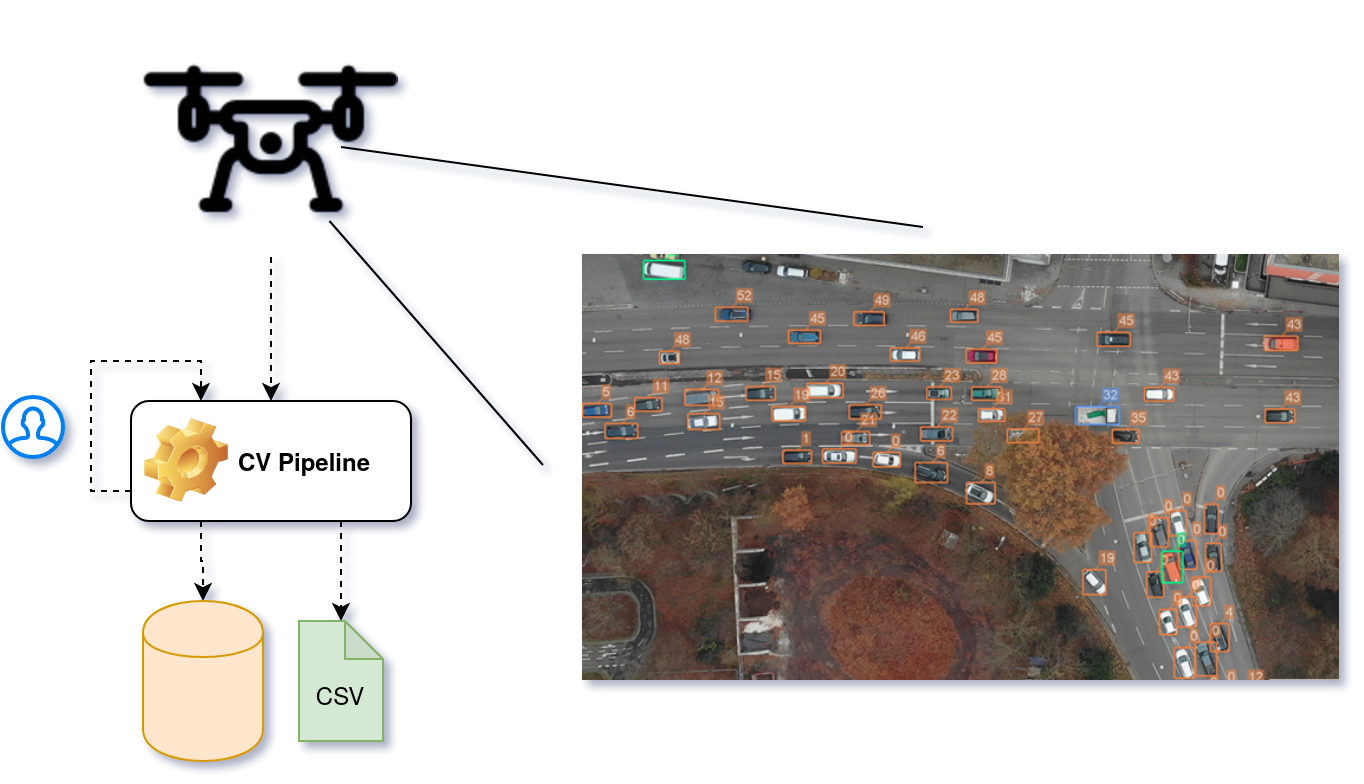
\includegraphics[width=0.9\textwidth]{overview_3.png}
	\caption{Overview of workflow}
\end{figure}

\section{Desired Workflow}
\label{workflow}
\label{workflow:desired:docker}

The desired workflow shall be supported through an user interface that provides an overview of all active projects and their current state, such as running computation, awaiting user input, failed or succeeded.

To create a new project, a predefined pipeline definition shall be selected as well as a name chosen.
Because only a handful of different pipeline definitions are expected, the creation of such does not need to happen through the user interface.
Instead, it is acceptable to have to manually edit a configuration file in such rare circumstances.

Once a project is created, the user wants to select the path to the input video.
This file has to be been uploaded to a global resource pool at this point.
The upload and download of files shall therefore also be possible through the user interface.
Because a video is usually recorded in 4k (3840 x 2160 pixels), encoded with H.264 and up to 20 minutes long, the upload must be capable of handling files which are tens of gigabytes large.

Once a pipeline is started, it shall execute the stages on the most fitting server node until finished, failed or a user input is required.
Throughout, the logs of the current and previous stage shall be accessible as well as uploading or downloading files from the current or previous stages workspace.
In addition to the pipeline pausing itself for user input, the user shall be able to request the pipeline to pause after the current stage at any moment.
When resuming the pipeline, the user might want to overwrite the starting point to, for example, redo the latest stage.

Mechanisms for fault tolerance shall detect unexpected program errors or failures of server nodes.
Server nodes shall be easily installed and added to the existing network of server nodes.
Each server node might provide additional hardware (such as GPUs), which shall be detected and provided.

For the ease of installation and binary distribution, Docker Images shall be used for running the Java Program for analyzing the videos as well the to be implemented management software.

%\todo{describe: project/pipeline -> stage?}




\section{Deliverable Requirements}

From the desired workflow, the following requirements can be extracted:

\begin{itemize}
	\item A user interface for interaction between the system and the user
	\item Storage management for global resource files as well as stage based workspaces
	\item Pipeline definition through configuration files
	\item Handling of multiple projects with independent progress and environment
	\item Reflecting the correct project state (running, failed, succeeded, paused)
	\item Log accumulation and archiving
	\item Accepting user input to update environment variables, resuming and pausing projects as well as uploading and downloading files into or from the global resource pool or a stages workspace.
	\item Assigning starting stages to the most fitting server node
	\item Detecting program errors (in a stage execution)
	\item Cope with node failures
	\item Using Docker Images as installation medium
	%Providing a Docker Image for the implemented program, preferably in an automated fashion.
%	\item \todo{.} Increase productivity without staff involvement
%	\item \todo{.} Utilize hardware in absence of staff
%	\item \todo{.} Decrease need of staff monitoring and organizing stuff
\end{itemize}

Further non-functional requirements are, that the user interface is to be implemented as Angular Web-Application using a REST API (for more details see \autoref{fundamental:angular}) for data transfer.
The system shall increase the productivity and hardware utilization, especially in times where the staff is absence.
The need to constantly monitor and interfere with the system to progress projects shall be decreased by providing automated mechanisms where possible and appropriate.

%\todo{mention? node failure resilient, easy to setup, decentralized?}

%\todo{something something agile extended as needed? \autoref{fundamental:agile}}

\begin{comment}
\subsection{Derived Requirements} \todo{.}
Requirements that are derived by looking at other requirements.


\todo{functional vs nonfunctional}

Die hier gelisteten funktionalen Anforderungen beschreiben das gewünschte Verhalten des
Systems \cite[155]{goll2012methoden}.

Nichtfunktionale Anforderungen zeigen im Gegensatz zu funktionalen Anforderungen Rah-
menbedingungen bei der Umsetzung des Systems auf \cite[155]{goll2012methoden}.
\end{comment}


\subsection{Non-Requirements}

To know the requirements and expectations of a system is essential, but knowing what is not expected by the system is at least as valuable.
It prevents wasting resources, efforts and architectural specializations that will never be required or in the worst case, make further development harder by restricting available choices for the future.
 
The system to implement shall not strive to implement real time scheduling or low latency scheduling.
The expected work items are big chunks that require hours to compute, whether the assignment of the work item takes sub-seconds or several seconds is nearly unnoticeable in the overall compute time.
\chapter{Outcome and Measurements}

In this chapter the outcome is measured and evaluated.

\todo{compare to initial deliverable requirements?}

\section{What did not work as expected}

\todo{timeout for events might be reached when in between the bandwidth is used by a copy of a large file and the extend signal is because of that deferred, stages that are fine are then marked as failed}

\todo{. old sections}

\section{User Authentication and Security}

One aspect that was not yet mentioned at all is user authentication and security.
Winslow is prepared in this regards because every project has an owner field and a member list and every web access check these.
An internal user repository also associates user with groups and provides defaults, such as the user and group \enquote{anonymous} and \enquote{root}, for no and full access privileges, respectively.
But at the moment, there is no user login, instead to the system all requests seem to be issued by \enquote{root}.
In the future this is planned to be replaced by an Single Sign-On implementation that uses the user accounts of our company.
Winslow is then associating a from this service given user name to an internal user and groups.
Unknown users are not allowed to see or alter anything, known users will be able to create and view their own projects and projects they are listed in as members.
%\todo{mostly planned, implemented not tested}

Winslow also supports secure HTTP (HTTPS) whenever a SSL certificate is provided\footnote{This can be seen in \autoref{appendix:winslow_installation}}.

\begin{comment}
\section{Storage}

One of the central concerns is the storage management.
The program needs to make input files available on each execution node and collect the results once the computation is complete.
There are a few main architectural strategies to approach this.
Simplified, either at a centralized location which is accessed by all execution nodes, a copy of the input files to the execution nodes or decentralized and distributed between all execution nodes and replication.
The advantages and disadvantages can depend on the specific implementation and is therefore discussed in combination of such (see \autoref{state_of_the_art}).

Further testing is required to decide whether a more complex storage system is required, or the simplicity of a centralized solution outweighs the setup and maintenance overhead.

%\subsection{Hadoop File System}
%\cite{hdfs:main}
%\cite{hdfs:doc}
%\todo{redudancy for evenly distributed}

%\subsection{NFS}
%
%local/per node cache?

\section{Coordination}

Another important concern is the coordination of the nodes.
A central coordinator with external server nodes, such as GitLab and Jenkins have, might not be sufficient for more complex and longer lasting pipelines.
The probability that the master would need to be offline while there is a stage executed, is in the scenario of the desired workflow higher than for GitLab or Jenkins, because the stage is being execution for hours or days.
Coupling stage execution plans on node availability ahead of time, as well as recovering from a sudden master failure implies additional implementation complexity.
A decentralized coordination needs to be able to do this as well, but also allows the usage of the system while a node failed or is unreachable due to maintenance.
With further prototyping and research a reasonable solution shall be found.

\section{Binary distribution}

In a time where containers are common and have proven to be usable, the installation of the binaries directly on the operating system they are executed on shall be avoided.
There shall be no manual, nor automatic but custom file copies of the binaries or images from one server to the other.
Experience shows, that without a proper management, this can easily become a mess, in which it is no longer clear, which files or images belong to which version.
At the same time, making all binaries publicly available through the Docker Hub\cite{docker:hub} is no option either.
Whether a self hosted Docker Registry\cite{docker:registry} could be the solution to this will be determined in further testing.

\section{User Interface}

Providing a useful user interface might not be important to the functionality of the system itself but for the user experience.
A bad user experience will cause a system not to be used.
It became common practice for a rich user experience to be web based and interactive with JavaScript.
For a potentially decentralized system, it is also advantageous to be able to access a disconnected node in the same manner as the remaining system, which further encourages a web based solution.
Web based solutions such as React and Angular shall therefore be investigated for being used as user interface.

\section{Requirements}

\todo{more than first defined - as expected}

\todo{lots more UI shortcuts found necessary while starting to use winslow}

\section{Architecture}

\todo{loosely coupled backend driver}\autoref{architecture:detailed}
\end{comment}

\section{High Level System Overview}

\todo{.delete?}

\autoref{architecture:high-level} shows the high level system overview of Winslow as it has been implemented by the end of this thesis.

\begin{figure}[h]
	\centering
	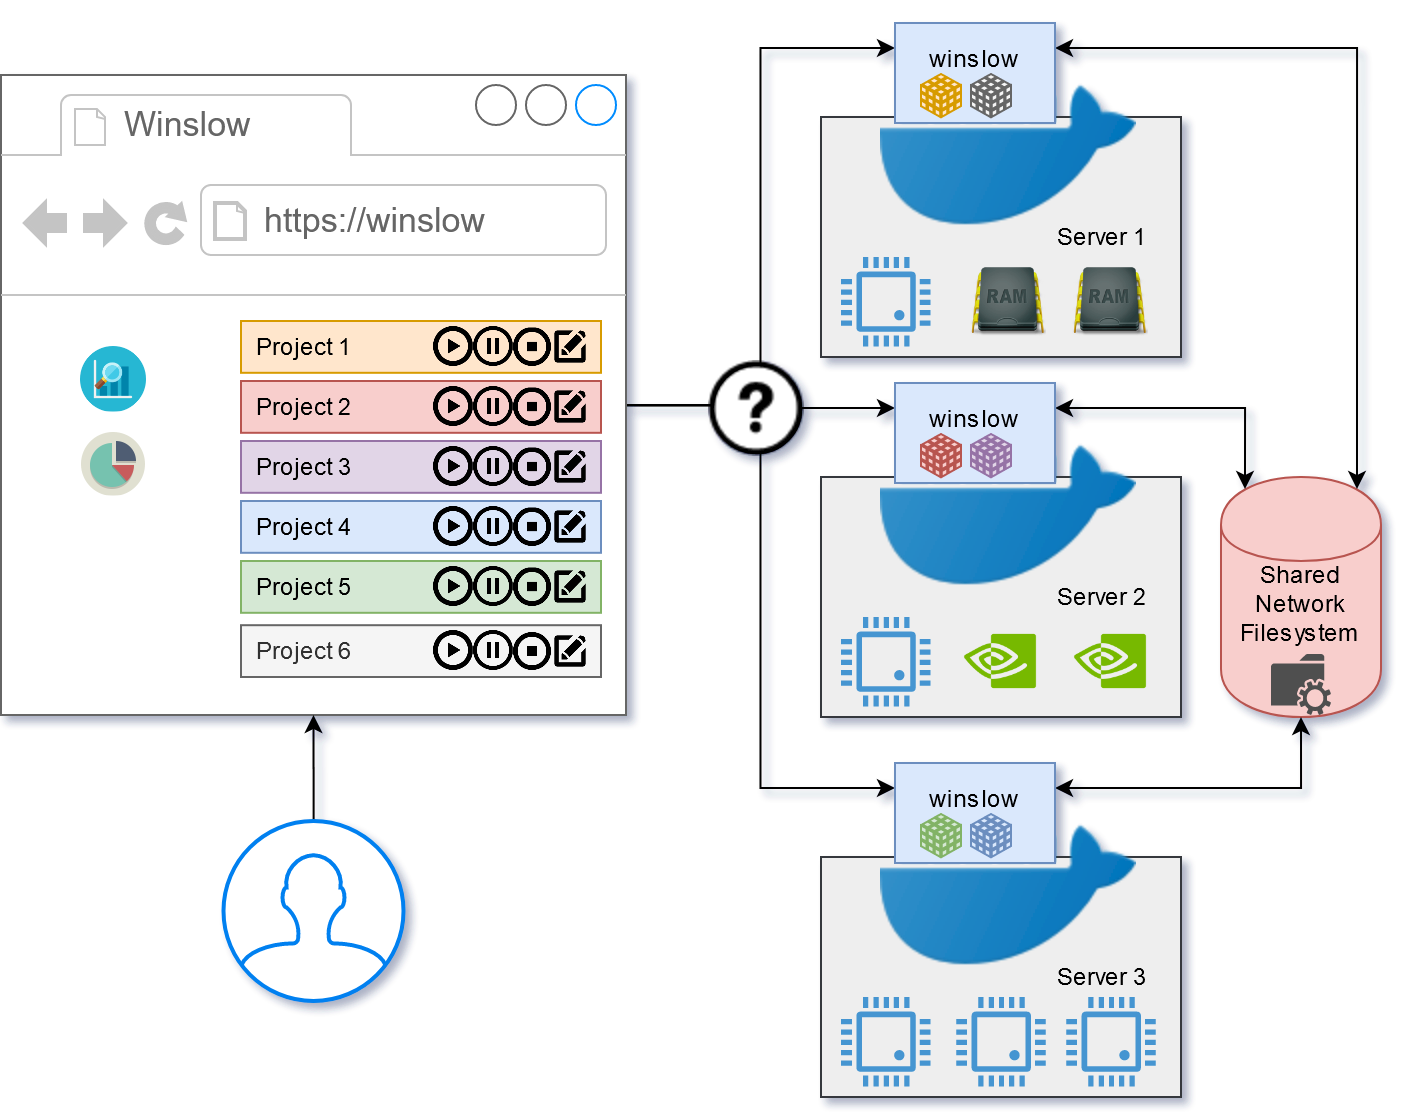
\includegraphics[width=0.8\textwidth]{architecture.png}
	\caption{High level view on the system structure}
	\label{architecture:high-level}
\end{figure}


\todo{explain what is going on in \autoref{architecture:high-level}}

\section{Failure resilience}

\todo{.delete? or polish!}

One of the initial requirements is to be resilient against node failures.
Node failures can be simulated easily by killing the Docker container of a Winslow instance.
The behaviour that is then displayed, depends on whether that killed instance was executing a stage.
If it did not, the only change is that in the Web-Application the node with its utilization reports will vanish.

But if it did execute a stage, it held locks for it.
These locks will expire, and after the additional grace period (see \autoref{message:grace_period}), the other instances will notice it, lock the affected project themselves and mark the execution as failed.
Currently, the project is then paused and user confirmation awaited.
An alternative to this could be to re-schedule the stage automatically.
\chapter{State of the art}

\section{Existing software solutions}

\subsection{Hadoop MapReduce}

focus transforming a big dataset by splitting it into many jobs, distributing it onto many workers, doing a transformation on each dataset, and merging it back together (only map -> reduce)
Distributed filesystem

\subsection{Quartz}

http://www.quartz-scheduler.org/
http://www.quartz-scheduler.org/overview/

\begin{itemize}
	\item + Java
	\item - requires integration
	\item - aimed towards running a job at a given time or in certain intervals
\end{itemize}

\subsection{Jenkins / GitLab}

Pipeline file with multiple stages
a stage can be executed on a host
focused on doing a job with different inputs again and again and again
CI -> usually no user interaction

\subsection{Camunda}

https://camunda.com/

Rich Business Process Management tool, many types of tasks, steps, transitions, triggers and endpoints.
Focused upon moving a dataset along the matching path of the process.
Out of the box graphical user interface for process definition and interaction.
Allows custom external worker through queues.
Misses capability to control which task to process on which worker through fine grained filters and how to allocate and distribute resources(?).

\section{Docker}

\chapter{Things to solve / decide upon}

\section{Programming language}

\subsection{Java}
\subsection{Rust}
\subsection{Scala?}
\subsection{Go?}

\section{Docker image packaging?}
\chapter{Implementation}

log strategy?

how to handle changes in configuration on a restart
 - how to sync with nomad
 - how to handle still running jobs on an now invalid configuration?
    - keep copy of old configuration?

\section{Orientation}

bash -> variable substitution

\section{No unexpected behavior}

no null, instead use Optional

lists are never null nor Optional but empty or filled instead

see de.itd.tracking.winslow.config.*

called defensive programming?
  - good to be error-resilient
  - bad in performance critical scenarios
  

%\include{chapters/ex4}
%\include{chapters/deliverables}

%---------------------------------------------------------------------
%--- Bibliography and appendices
%---------------------------------------------------------------------

\printbibliography
\addcontentsline{toc}{chapter}{Bibliography}

%\appendix
%% to utf8: ö
\chapter{Extra data}

		
\end{document}
